\documentclass{beamer}
\usetheme{metropolis} % Use the metropolis theme

% Add tikz and pgfplots packages
\usepackage{tikz, pgfplots}
\usetikzlibrary{positioning}

% For clicking references
\usepackage{hyperref}

% For better horizontal lines
\usepackage{booktabs}

% For better referencing
\usepackage{cleveref}

\usepackage{graphicx}


\usepackage{amsmath}

\usepackage{wasysym}

% Define custom pastel colors
\definecolor{pastelRed}{RGB}{255, 105, 97}   % A soft pastel red
\definecolor{pastelBlue}{RGB}{119, 158, 203} % A muted pastel blue
\definecolor{pastelYellow}{RGB}{255, 223, 0} % A gentle pastel yellow
\definecolor{lightGray}{RGB}{211, 211, 211}  % A light gray for subtitles and less emphasized text

% Apply the custom colors
\setbeamercolor{palette primary}{bg=black, fg=white}
\setbeamercolor{palette secondary}{bg=lightGray, fg=black}
\setbeamercolor{palette tertiary}{bg=black, fg=white}
\setbeamercolor{titlelike}{parent=palette primary, fg=black}
\setbeamercolor{subtitle}{fg=lightGray}
\setbeamercolor{structure}{fg=black} % For itemize, enumerate, etc

% Change color of normal text
\setbeamercolor{normal text}{fg=black, bg=white}

% Set the color of the table of contents
\setbeamercolor{section in toc}{fg=black} % Section titles in TOC
\setbeamercolor{subsection in toc}{fg=black} % Subsection titles in TOC

% Set block colors
\setbeamercolor{block title}{use=structure,fg=white,bg=pastelRed}
\setbeamercolor{block body}{fg=black,bg=white}



% Title Page Info
\title{Misc}
\subtitle{Ting vi ikke gik igennem, eller ikke er en del af spørgsmålene}
\author{Kevin Vinther}
\date{\today}

\begin{document}

% Title Page
\begin{frame}
  \titlepage
\end{frame}

% Table of Contents
\begin{frame}[allowframebreaks]
  \frametitle{Table of Contents}
  \tableofcontents
\end{frame}

\section{Misc 1}
\label{sec:misc1}



\subsection{Notes on combinatorial proofs}
\label{sec:weeklynote2}

\begin{frame}[allowframebreaks]
  \frametitle{Notes on Combinatorial Proofs}
 \begin{itemize}
 \item Det her er bare et simpelt kombinatorisk bevis af Jørgen. 
 \end{itemize} 
 \begin{theorem}
If $S$ is a finite set with at least one element, then the number of even subsets of $S$ is the same as the number of odd subsets of $S$.
 \end{theorem}
 \begin{itemize}
 \item Der kommer to beviser. 
 \item Først, læg mærke til at dette ikke gælder når $S = \emptyset$.
 \item Lad $E_{S}$  være antallet af lige subsets og $O_{S}$ antallet af ulige subsets af S. 
 \item Sidst, lad $n = |S|$ (i.e., kardinaliteten af $S$.)
 \item \textbf{Første bevis:}
 \item Der er præcis $\binom{n}{k}$ måder at vælge et sæt med $k$ elementer fra $S$.
 \item Husk binomial theorem: $(x+y)^{n} = \sum_{k=0}^{n} \binom{n}{k}x^{n-k}y^{ k}$.
 \item Hvis vi siger at $x = 1$ og $y = -1$ får vi $0 = \sum_{k=0}^{n} \binom{n}{k} (-1)^{k}$. 
 \item Vi kan dermed se at hvert lige subset bliver 1, og hvert ulige bliver -1.
 \item \textbf{Andet bevis:}
 \item Teoremet holder klart når $n=1$, så tænk på et sæt $S$ med $n > 1$ elementer. 
 \item Vi ``fikser'' et element $s \in S$ og lader $S' = S \setminus \{s\}$. 
 \item Lad $e_{s}, o_{s}$ være antallet af lige og ulige subsets af $S$ som indeholder $s$ (dvs. det tal vi ``fiksede'' før.)
 \item Hvert lige (ulige) subset af $S$ som har $s$ i sig, har $s$ plus et ulige (lige) subset af $S'$. 
 \item Dermed har vi $e_{s} = O_{S'}$ og $o_{s} = E_{S'}$. 
 \item Til sidst, observér at, gennem sum-reglen, antallet af lige (ulige) subsets fa $S$ er lig med antallet af lige (ulige) subsets der indeholder $s$ plus antallet af lige (ulige) subsets af $S$ der ikke indeholder $s$. 
 \item Dermed: \[ E_{S} = e_{s} + E_{S'} = O_{S'} + E_{S'} = O_{S'} + o_{s} = O_{S} \]
 \end{itemize}
\end{frame}

\begin{frame}[allowframebreaks]
  \frametitle{Andet teorem}
 \begin{itemize}
 \item Vi giver nu endnu et eksempel af hvordan kombinatoriske argumenter kan bruges.
 \item For givne heltal $k,n$ lader vi $S_{n,k} = \{(n_{1}, n_{2}, \ldots, n_{k}) | n_{i} \geq 0 \text{ og } n_{1} + n_{2} + \cdots + n_{k} = n\}$
 \item Læg mærke til at $S_{n,k}$ er sættet af alle ordnet (ordered) $k$-tupler, med et ikke-negativt tal for hvilke summen af elementerne i tuplen er $n$. 
 \item Fra Rosen 6.5.3 ved vi at der er $\binom{n+(k-1)}{n}$ af disse.
 \end{itemize} 
 \begin{theorem}
\[ \sum_{(n_{1}, n_{2}, \ldots, n_{k}) \in S_{n,k}}^{} \frac{n!}{n_{1}! \cdot n_{2}! \cdot \cdots \cdot n_{k}!} = k^{n} \]
\end{theorem}
\begin{itemize}
\item \textbf{Bevis:}
\item Vi påstår at begge sider af lighedstegnet tæller antallet af måder at distribuere $n$ distinkte bolde i $k$ distinkte bokse. 
\item Det er nemt at se på højresiden: vi har $k$ valg for hver af de $n$ bolde, så $k^{n}$ i alt. 
\item For venstresiden tæller vi det samme. Af Rosen Theorem 4 side 452 ved vi at for fiksede $n_{1}, n_{2}, \ldots, n_k$ således at $\sum_{i=1}^{k} n_{i} = n$ er der $\frac{n!}{n_{1}! \cdot n_{2}! \cdot \cdots \cdot n_{k}!}$ måder at distribuere dem.
\end{itemize}
\end{frame}

\subsection{Kombinatoriske Beviser (Rosen 6.3)}
\label{subsec:rosen63}

\begin{frame}[allowframebreaks]
  \frametitle{Kombinatoriske Beviser}
  \begin{itemize}
  \item Håber I er klar gutter!
  \end{itemize}
  \begin{definition}
A \textit{combinatorial proof} of an identity is a proof that uses counting arguments to prove that both sides of the identity count the same objects but in different ways or a proof that is based on showing that there is a bijectino between the sets of objects counted by the two sides of the identity. These two types of proofs are called \textit{double counting proofs} and \textit{bijective proofs} respectively.
  \end{definition}
  \begin{itemize}
  \item Så, med \textbf{dobbelttælningsbeviser} er målet af vise at begge sider af en identitet i essensen tæller det samme sæt af objekter (se f.eks. $\binom{n}{k} = \binom{n}{n-k}$).
  \item Et \textbf{bijektivt bevis} arbejder ved at etablere en en-til-en korrespondance mellem de to sæt, som tælles. Det skal bekræftes at hvert element i et sæt svarer \textbf{præcist} til et objekt i et andet sæt. Hvis dette gælder, tæller de det samme, og er dermed lig hinanden. 
  \item Lad os, for eksempel, kigger på beviserne for $\binom{n}{r} = \binom{n}{n-r}$. 
  \item Antag at $S$ er et sæt med $n$ elementer. 
  \item Funktionen som ``mapper'' et subset $A$ af $S$ til $\overline{A}$  er en bijketion mellem subsetsne af $S$ med $r$ elementer, og subsetsne med $n-r$ elementer.
  \item Du kan tænke på det på den her måde: For hvert sæt der bliver talt i $A$ bliver der udeladt et antal af elementer, $|\overline{A}|$. 
  \item Disse elementer bliver undlandt lige så mange gange, som du tæller de originale tal.
  \item \textbf{Dobbelttælningsbevis}:\footnote{jeg tænker bare jeg skriver double countign fra nu af, det er godt nok irriterende at skrive et så langt ord.} Af deginitionen er antallet af subsets af $S$ med $r$ elementer $\binom{n}{r}$. Men hvert subset $A$ af $S$ bliver også valgt ved at specificere hvilke elementer der \textbf{ikke} er en del af $A$ og dermed er i $\overline{A}$. 
  \end{itemize}
  \begin{theorem}[1. The Binomial Theorem]
    Let $x$ and $y$ be variables, and let $n$ be a nonnegative integer. Then
    \[ (x+y)^{n} = \sum_{j=0}^{n} \binom{n}{j} x^{n-j}y^{j} = \binom{n}{0}x^{n} \binom{n}{1}x^{n-1}y + \cdots + \binom{n}{n-1}xy^{n-1} + \binom{n}{n} y^{n} \]
  \end{theorem}
  \begin{itemize}
  \item Vi beviser kombinatorisk. 
  \item Leddene i produktet, når de bliver udvidet, er af formen $x^{n-j}y^{j}$ for $j = 0, 1, 2, \ldots, n$. 
  \item For at tælle antallet af led af formen $x^{n-j}y^{j}$, notér at for at få sådan et led skal man vælge $n-j$ $x'$er fra de $n$ binnomiale faktorer (således at de andre $j$ led i produktet er $y$'er). 
  \item Dermed er koefficienten af $x^{n-j}y^{j} = \binom{n}{n-j}$, hvilket er lig med $\binom{n}{j}$. Dette beviser teoremet. 
  \end{itemize}
  \begin{theorem}[2. Pascal's Identity]
Let $n$ and $k$ be positive integers with $n \geq k$. Then \[ \binom{n+1}{k} = \binom{n}{k-1} + \binom{n}{k} \].
  \end{theorem}
  \begin{itemize}
  \item Igen beviser vi kombinatorisk (haha, man skulle næsten tro at det var målet med den her fremlæggelse.)
  \item Antag at $T$ er et sæt tilhørende $n+1$ elementer. 
  \item Lad $a$ være et element i $T$ og lad $S = T - \{a\}$.
  \item Læg mærke til at der er $\binom{n+1}{k}$ subsets af $T$ med $k$ elementer. 
  \item (igen, $n+1$ fordi $T$ er defineret, ikke til at have $n$ elementer, men $n+1$)
  \item Et subset af $T$ med $k$ elementer indeholder enten $a$ sammen med $k-1$ elementer af $S$, eller $k$ elementer af $S$ og inderholder ikke $a$.
  \item Fordi der er $\binom{n}{k-1}$ subsets af $k-1$ elementer af $S$, er der $\binom{n}{k-1}$ subsets af $k$ elementer af $T$ der indeholder $a$. 
  \item Der er $\binom{n}{k}$ subsets af $k$ elementer af $T$ som ikke indeholder $a$, fordi der er $\binom{n}{k}$ subsets af $k$ elementer af $S$.
  \item Dermed teoremet.
  \end{itemize}
  \begin{theorem}[3. Vandermonde's Identity]
    Let $m, n$ and $r$ be nonnegative integers with $r \leq m, n$. Then
    \[ \binom{m+n }{r} = \sum_{k=0}^{r} \binom{m}{r-k} \binom{n}{k}  \]
  \end{theorem}
  \begin{itemize}
  \item Antag at der er $m$ elementer i et sæt, og $n$ i et andet. 
  \item Så er der i alt $\binom{m+n }{r}$ måder at vælge $r$ elementer fra begge sæt.
  \item En anden måde at vælge $r$ elementer fra fællesmængden er at vælge $k$ elementer fra det andet sæt, og så $r-k$ elementer fra det første sæt, hvor $k$ er et heltal $0 \leq k \leq r$. 
  \item Fordi der er $\binom{n}{k}$ måder at vælge $k$ elementer fra det andet sæt på, og $\binom{m}{r-k}$ måder at vælge $r-k$ elementer fra det første sæt, fortæller product rule os at det kan blive gjort på $\binom{m}{r-k} \binom{n}{k}$ måder. 
  \item Dermed er det fulde antal af måder du kan vælge $r$ elementer på fra fællesmængden lig med \[ \sum_{k=0}^{r} \binom{m}{r-k} \binom{n}{k} \]
  \item Vi har fundet du udtryk for antallet af måder at vælge $r$ elementer på fra fællesmængden af et sæt med $m$ elementer, og et sæt med $n$ elementer. 
  \item Dette beviser Vandermonde's Identitet
    \end{itemize}
    \begin{theorem}[4]
      Let $n$ and $r$ be nonnegative integers with $r \leq n$. Then
      \[ \binom{n+1}{r+1} = \sum_{j=r}^{n}\binom{j}{r} \]
    \end{theorem}
    \begin{itemize}
    \item Et tidligere eksempel har vist at $\binom{n+1}{r+1}$ tæller antallet af bit-strenge af længde $n+1$ der har $r+1$ et'taller
    \item Vi vil vise at højresiden tæller de samme objekter ved at se på antallet af korresponderende mulige lokationer af det sidste 1 i en streng med $r+1$ 1'ere. 
    \item Det sidste 1 må være ved position $r+1, r+2, \ldots, \text{ eller } n+1$. 
    \item Ydermere, hvis det sidste et er det $k$'e bit, må der være $r$ et'ere imellem de første $k-1$ positioner. 
    \item Vi ved at der er $\binom{k-1}{r}$ af disse slags bitstrenge. 
    \item Hvis vi summerer over $k$ med $r + 1 \leq k \leq n + 1$, finder vi at der er
      \[ \sum_{k=r+1}^{n+1} \binom{k-1}{r} = \sum_{j=r}^{n} \binom{j}{r} \]
      bit strenge af længde $n$ med præcis $r+1$ et'taller.
    \end{itemize}
\end{frame}

\subsection{Recurrence Relations}
\label{subsec:recurrencerelations}

\begin{frame}
  \frametitle{Recurrence Relations}
 \begin{itemize}
 \item En recurrence relation er en rekursiv definition med mere end et initial term. 
 \item En sekvens er en løsning af recurrence relationen hvis dets led satisfy relationen. 
 \item \textbf{Eksempel med fibonacci:} $f_{n} = f_{n-1} + f_{n-2}, n \geq 3, f_{1} = 1, f_{2} = 1$.
 \item \textbf{Eksempel: Tower of Hanoi}
 \end{itemize} 
\end{frame}

\begin{frame}[allowframebreaks]
  \frametitle{Algorithms and Recurrence Relations}
 \begin{itemize}
 \item Recurrence Relations kan bruges til at finde kompleksiteten af divide-and-conquer algoritmer. 
 \item Vi introducerer nu \textbf{Dynamic Programming}. 
 \item Dynamic Porgramming er et paradigme en algoritme følger, hvis den rekursivt ``breaker down'' et problem i mindre, men overlappende subproblemer, og så udregner løsningne ved brug af løsningerne af subproblemerne. 
 \end{itemize} 
\end{frame}

\begin{frame}[allowframebreaks]
  \frametitle{Solving Linear Recurrence Relations}
  \begin{itemize}
  \item En vigtigt klasse af recurrence relations kan blive løst på en systematisk måde. 
  \end{itemize}
  \begin{definition}
    A \textit{linear homogeneous recurrence relation of degree $k$ with constant coefficients} is a recurrence relation of the form

    \[ a_{n} = c_{1}a_{n-1} + c_{2}a_{n-2} + \cdots + c_{k}a_{nk} \]
    where $c_{1}, c_{2}, \ldots, c_{k}$ are real numbers, and $c_{k} \neq 0$.
  \end{definition}
  \begin{itemize}
  \item Den er \textbf{lineær} fordi højresiden er summen af de tidligere led af sekvensen, hvert led ganget med en funktion af $n$. 
  \item Den er \textbf{homogen} fordi ingen led forekommer som er multiplum af $a_{j}$'erne. 
  \item Koefficienterne i sekvensen er alle \textbf{konstanter}, i stedet for funktioner der afhænger af $n$.
  \item \textbf{Degreeen} (dansk?) er $k$ fordi $a_{n}$ er udtrykt ved brug af de tidligere $k$  led i sekvensen. 
  \end{itemize}
\end{frame}

\begin{frame}
  \frametitle{Eksempel på linear recurrence}
  $P_{n} = (1.11)P_{n-1}$ er et eksempel på en homogen rekursionsligning (siger chatgpt det hedder på dansk, ret mig lige hvis jeg tager fejl). Ligningen har ``degree'' 1.
  Fibonacci $f_{n} = f_{n-1} + f_{n-2}$ er også lineær, men med en degree på to.
  $a_{n} = a_{n-5}$ har en degree af 5.
\end{frame}

\subsection{Weekly Note 6 Note}
\label{subsec:week6}

\begin{frame}[allowframebreaks]
  \frametitle{Conenction between Stirling Numbers and the number of onto functions}
  \begin{itemize}
  \item Stirling Numbers $S(m,n)$ er antallet af måder man kan distribuere $m$ distinguishable elementer i $n$ ikke-distinguishable bokse, således at hver boks har mindst et element. 
  \item VI laver en onto funktion fra et sæt $X$ af $m$ elementer og et sæt $Y$ af $n$ elementer. 
  \item Tænk på et andet problem hvor vi har $n$ bokse der kan skælnes mellem, navngivet 1, 2, n. Ignorer derefter navnene
  \item Derefter gør følgenede: 
    
    \begin{enumerate}
    \item Distribuer elementer fra $X$ i de $n$ bokse så der er ingen tomme
    \item Kig på navnene af boksene og få en funktion $f$ fra $X$ til $Y$ ved at mappe et element $x \in X$ til $y_{i}$ hvis det var palceret i boksen hvis navn fra $i$. 
    \end{enumerate}
    \item På denne måde, for hver måde man kan lave step 1 på, er der $n!$ onto funktioner, nemlig antallet af måder vi kan navngive de $n$ bokse. 
    \item Dette viser at antallet af onto funktioner fra et sæt med $m$ elementer til et sæt af $n$ elementer er præcis $n! \cdot S(m,n)$
    \item Det følger dermed at:
    \[ S(m,n) = \frac{1}{n!} \left[ n^{m} - \binom{n}{1}(n-1)^{m} + \binom{n}{2}(n-2)^{m} - \cdots + (-1)^{n-1} \binom{n}{n-1} \right] \]
  \end{itemize}
\end{frame}

\subsection{Probabilistic Method: Ramsey Number}
\label{subsec:ramsey}

\begin{frame}[allowframebreaks]
  \frametitle{Ramsey Number}
  \begin{itemize}
  \item Den probabilistiske metode er en teknik brugt til at lave nonkonstrutive eksistensbeviser.
  \item Nonkonstruktiv = Du viser ikke hvordan man finder elementet 
  \item Eksistensbevis = du beviser at elementet eksisterer
  \item For at bevise at et element i et sæt $S$  eksisterer, giver vi sandsynligheder til elementerne i $S$ med en specifik property. 
  \item Vi kan så vise at et element eksisterer ved at vise at sandsynligheden for at $x \in S$ har en property er positiv. 
\end{itemize}
\begin{theorem}[3. The Probabilistic Method]
If the probability that an element chosen at random from a $S$ does not have a particular property is less than 1, there exists an elementin $S$ with this property.
\end{theorem}
\begin{itemize}
\item Det er herfra tydeligt at se hvorfor et bevis baseret på probabilistic method er nonkonstruktivt.
\item Før vi viser et lower bound på Ramsey refreshes Ramsey Number.
\end{itemize}
\end{frame}

\begin{frame}[allowframebreaks]
  \frametitle{Ramsey Numbers}
  \begin{itemize}
  \item Ramsey Tallet $R(m,n)$ hvor $m$ og $n$ er positive heltal større end eller lig med 2, er det minimum antal af personer til en fest således at der er enten $m$ fælles venner eller $n$ fælles fjender. 
  \end{itemize}
  \begin{example}[13]
Assume that in a group of six people, each pair of individuals consists of two frients or two enemies. Show that there are either three mutual friends or three mutual enemies in the group. 
\end{example}
\begin{itemize}
\item Altså, for hvert par af 2 personer kan de enten være fjender eller venner. 
\item Eksempler siger at vi skal vise at i en gruppe af 6 personer er der enten 3 fælles venner eller 3 fælles fjender. 
\item Løsning:
\item Lad $A$ være en af de 6 personer. 
\item Af de andre 5 personer i gruppen er der enten 3 eller flere som er venner af $A$, eller tre eller flere som er fjender af $A$. 
\item Dette følger fra dueslagsprincippet. $\lceil 5/2 \rceil = 3$
\end{itemize}
\end{frame}

\begin{frame}[allowframebreaks]
  \frametitle{Bound v.h.a Probabilistic Method}
  \begin{theorem}[4]
If $k$ is an integer with $k \geq 2$, then $R(k,k) \geq 2^{k/2}$
\end{theorem}
\begin{itemize}
\item Bevis: 
\item Vi ved at teoremet holder ved $k = 2$ og $k = 3$ fordi $R(2,2) = 2$ og $R(3,3) = 6$, som vist tidligere. Antag nu at $k \geq 4$. 
\item Vi vil bruge probabilistik metode til at vise at hvis der er færre end $2^{k/2}$ personer til en fest, er det muligt at ingen af de $k$ er fælles venner eller fælles fjender, dermed kan vi konkludere at $R(k,k) \geq 2^{k/2}$.
\item Vi antager at chancen for at to venner er fjender er lig chancen for at to personer er venner.
\item Antag at der er $n$ personer til festen. 
\item Det følger at der er $\binom{n}{k}$ forskellige sæt af $k$ personer til denne fest. 
\item Vi lader det skrives $S_{1}, S_{2}, \ldots, S_{\binom{n}{k}}$.
\item Lad $E_{i}$ være begivenheden at alle $k$ personer i $S_{i}$ er enten fælles venner eller fælles fjender. 
\item Sandsynligheden at der er enten $k$ fælles venner eller $k$ fælels fjender imellem de $n$ personer er lig $p(\bigcup\limits_{i=1}^{\binom{n}{k}}E_{i})$
\item Ifølge vores antagelse er der lige sandsynlighed for to personer til at være venner eller fjender. 
\item Ydermere er der $\binom{k}{2} = k(k-1)/2$ par af personer i $S_{i}$ fordi der er $k$ personer i $S_{i}$. 
\item Dermed er sandsynligheden for at alle $k$ personer i $S_i$ er fælles venner og resp. fælles fjender $(1/2)^{k(k-1)/2}$. 
\item Det følger at $P(E_{i}) = 2(1/2)^{k(k-1)/2}$
\item Dermed er sandsynligheden for at der er enten $k$ fælles venner eller $k$ fælles fjender i en gruppe af $n$ personer lig med $p(\bigcup\limits_{i=1}^{\binom{n}{k}}E_{i})$.
\item Hvis vi bruger Sum Bound får vi at: \[ p \left( \bigcup\limits_{i=1}^{\binom{n}{k}}E_i \right) \leq \sum_{i=1}^{\binom{n}{k}} p(E_{i}) = \binom{n}{k} \cdot 2 \left( \frac{1}{2} \right)^{k(k-1)/2}\]
\item Fra en tidligere exercise (21, 6.4) Har vi at $\binom{n}{k} \leq n^{k}/2^{k-1}$. Dermed: \[ \binom{n}{k} 2 \left( \frac{1}{2} \right)^{k(k-1)/2} \leq \frac{n^{k}}{2^{k-1}}2 \left( \frac{1}{2} \right)^{k(k-1)/2}\]
\item Vi vil gerne vise at $R(n,n) \leq 2^{n/2}$ dermed, hvis vi antager at $n < 2^{k/2}$ har vi at \[ \frac{n^{k}}{2^{k-1}}2 \left( \frac{1}{2} \right)^{k(k-1)/2} < \frac{2^{k(k/2)}}{2^{k-1}}2 \left( \frac{1}{2} \right)^{k(k-1)/2} = 2^{2-(k/2)} \leq 1 \]
\item Det sidste led følger fordi $k \geq 4$.
\end{itemize}
\end{frame}

\subsection{Linearity Of Expectation}
\label{subsec:label}

\begin{frame}[allowframebreaks]
  \frametitle{Linearity of Expectations}
  \begin{theorem}[3]
    Let \(X_{i}, i = 1, 2, \ldots, n\) with \(n\) a positive integer, be random variables on \(S\), and let \(a\) and \(b\) be real numbers. Then:
    \begin{itemize}
      \item[(i)] \(E(X_{1}+X_{2}+\cdots+X_{n}) = E(X_{1}) + E(X_{2}) + \cdots + E(X_{n})\)
      \item[(ii)] \(E(aX+b) = aE(X)+b\)
    \end{itemize}
  \end{theorem}
  \begin{itemize}
    \item Vi fokuserer på (ii).
  \end{itemize}

  \begin{equation}
    \begin{split}
      E(aX  + b) &= \sum_{s \in S} p(s)(aX(s)+b)\\
                 &= a \sum_{s \in S} p(s)X(s) + b \sum_{s \in S} p(s) \\
                 &= aE(X)+b \quad \text{because} \quad \sum_{s \in S} p(s) = 1\\
    \end{split}
  \end{equation}
\end{frame}

\subsection{Independent Random Variables}

\begin{frame}[]
  \frametitle{Theorem 5 7.4}
  \begin{theorem}
    If \(X\) and \(Y\) are independent random variables on a sample space \(S\), then \(E(XY) = E(X)E(Y)\).
  \end{theorem} 
\end{frame}

\begin{frame}
  \frametitle{bevis}
 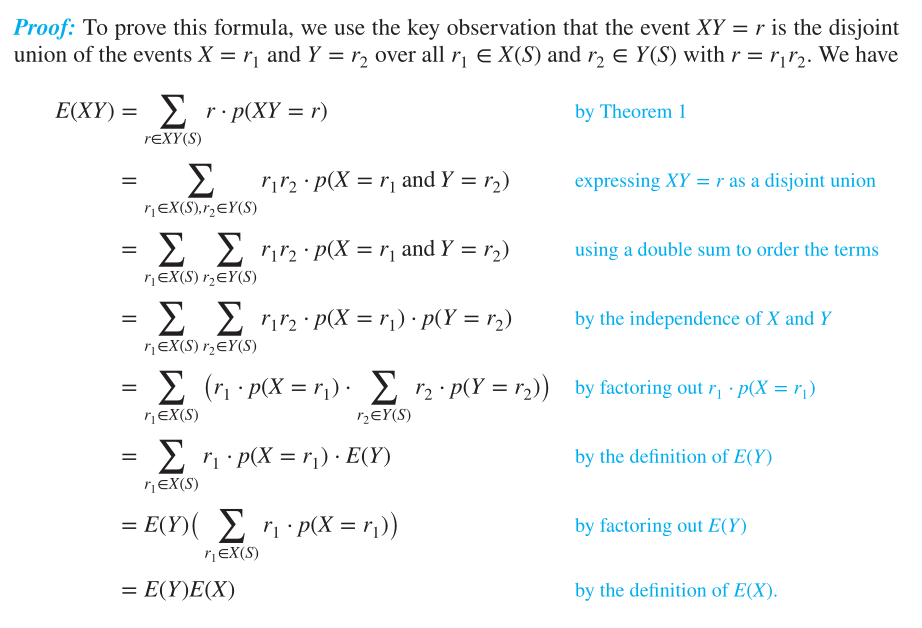
\includegraphics[width=340pt]{main--misc-1--linearity-of-expectation-7939.png} 
\end{frame}

\section{Misc 2}
\label{sec:label}



\subsection{Chernoff Bounds}
\label{subsec:label}

\begin{frame}[allowframebreaks]
  \frametitle{Chernoff Bounds}
  \begin{itemize}
  \item :(
  \item Lad $X$ være et random variable som er summen af flere uafhængige $0-1$-værdi random variables: $X = X_{1} + X_{2} + \cdots + X_{n}$ hvor $X_{i}$ tager værdien $1$ med sandsynlighed $p_{i}$ og 0 ellers. 
  \item Vi ved at $E(X) = \sum_{i=1}^{n}p_{i}$. 
  \item Intuitivt, siden $X_{i}$ er uafhængige, tænker man nok at de vil ``cancel out'' så deres sum er lig deres expected value med ret stor sandsynlighed. 
  \item Vi bruger Chernoff Bounds til at finde denne sandsxynlighed.
  \item Det kan finde sandsynligheden for både et upper og lower bound. 
  \end{itemize}
\begin{theorem}
  Let $X, X_{1}, X_{2}, \ldots, X_{n}$ be defined as above, and assume that $\mu \geq E(X)$. Then, for any $\delta > 0$, we have
  \[P(X > (1+\delta)\mu) < \left[ \frac{e^{\delta}}{(1+\delta)^{(1+\delta)}} \right]^{\mu}\]
\end{theorem}
\begin{itemize}
\item Så, i sin essens, er Chernoff Bounds sandsynligheden for at en værdi deviater meget fra $E(X)$.
\item $\mu$ er oftest bare $E(X)$ (very often, ifølge Jørgen), så længe $\mu \geq E(X)$ er det ok.
\item Givet følgende observation: \[ \forall t > 0 \; \; p(X > (1 + \delta) \mu) = p(e^{tX} > e^{t(1+\delta)\mu}) \] da $e^{ty}$ er monotont increasing med $y$ (altså, når $y$ bliver større, bliver hele værdien større).
\item Så dermed siger den bare at sandsynlighederne er de samme, da vi erstatter $y$ med hhv. $X$ og $(1 + \delta) \mu$.
\item Så; hvorfor gider vi gøre det endnu mere kompliceret at kigge på? 
\item Fordi den eksponentielle funktion har nogle dejlige properties vi kan bruge.
\item Vi ved fra Markov's inequality at \[ p(Y > \gamma) \leq \frac{E(Y)}{\gamma} \] og \[ \gamma p(Y > \gamma) \leq E(Y) \]
\item Fra dette kan vi finde: \[ p(X > (1+ \delta) \mu) = p(e ^{tX} > e^{t(1+ \delta) \mu}) \leq e^{t(1+ \delta) \mu} E[e^{tX}] \]
\item Nu vil vi så gerne bounde $E[e^{tX}]$: \[ E(e^{tX}) = E(e^{t \sum x_{i}} = E(e^{\sum t X_{i}}) = E( \prod_{i=1}^{n}e^{tX_{i}}) = \prod_{i=1}^{n} E(e^{tX_{i}}) \]
\item Siden $X_{i}$ er et indicator random variable \[ E(e^{tX_{i}}) = p_{i} \cdot e^{t}+ (1-p_{i}) \cdot e^{t\cdot 0} = p_{i}e^{t} + (1-p_{i}) = 1 + p_{i}(e^{t}-1) \]
\item Så \[ E(e^{tX_{i}}) \leq e^{p_{i} (e^{t}-1} \]
\item Da \[ 1 + x \leq e^{x} \] så længe $x \geq 0$
\item Nu har vi et upper bound. Det vil vi gerne sætte ind:  
\end{itemize}

\begin{equation}
\begin{split}
  E(e^{tX}) = \prod_{i=1}^{n}e^{tX_{i}} &\leq \prod_{i=1}^{n} e^{P_{i}(e^{t}-1} \\
                                    &= e^{\sum p_{i} (e^{t}-1}\\
                                    &= e^{(e^{t}-1) \Sigma p_{i}}\\
  &\leq e^{(e^{t}-1)\mu}
\end{split}

\end{equation}

\begin{itemize}
\item Fordi $\sum_{}^{}p_{i} = E(X) \leq \mu$
\item Vi kan nu få det ind således at $p(X > (1 + \delta) \mu) \leq e^{-t(1 + \delta) \mu} \cdot E(e^{tX})$
\item Vi sætter $p(X > (1+\delta)\mu) \leq e^{-t (1+\delta) \mu} \cdot e^{(e^{t}-1)\mu}$
\item Dette holder for alle $t > 0$, så hvis $t = \ln (1+ \delta)$ får vi 
\end{itemize}


\begin{equation*}
  \begin{split}
    p(X > (1 + \delta) \mu) &\leq e^{-\ln(1 + \delta) \cdot (1 + \delta) \mu} \cdot e^{(e^{\ln (1 + \delta)}-1) \mu}\\
                     &= (1+ \delta)^{-(1+ \delta) \mu} \cdot e^{(1 + \delta-1) \mu}\\
    &= \left[ \frac{e^{\delta}}{(1+\delta)^{(1+\delta)}} \right]^{\mu}
  \end{split}
\end{equation*}

\begin{itemize}
\item Og det var beviset:)
\item Men vi er ikke færdige!
\item Det kan også vises at $X$ er langt mindre (lower bound). \[ p(X < (1 - \delta) \mu) < e^{- \frac{1}{2}\mu \delta^{2}} \]
\item Nogle formler der er nemmere at bruge: \[ p(X > (1 + \delta) \mu) \leq e^{- \frac{\delta}{3}^{2}} \mu \text{ når } 0 < \delta \]
  \[ p(X < (1- \delta) \mu ) \leq e^{- \frac{\delta}{2}^{2}}\mu \text{ når } 0 < \delta < 1 \]
\end{itemize}
\end{frame}

\subsection{Contention Resolution}
\label{subsec:label}

\begin{frame}[allowframebreaks]
  \frametitle{The Problem}
 \begin{itemize}
 \item Antag at vi har $n$ processer, $P_{1}, P_{2}, \ldots, P_{n}$, hver af dem konkurrerer for adgang til en delt database. 
 \item Vi antager at tiden er opdelt i \textit{runder}. 
 \item Databasen har den egenskab at den kun kan blive accessed af én process per runde, og hvis mere end én proces forsøger så er alle låst ude.
 \item Så, vi vil gerne have så mange som muligt til at få adgang, men der er ingen grund til at få alle til det på en gang. 
 \item Hvordan finder vi så en algoritme når ingen af processerne kan kommunikere med hinanden? 
 \end{itemize} 
\end{frame}

\begin{frame}[allowframebreaks]
  \frametitle{Design af algoritmen}
 \begin{itemize}
 \item For en given proces $P_{i}$ og en given runde $t$, lad $A[i, t]$ være hændelsen at $P_{i}$ forsøger at få adgang til databasen i runde $t$. 
 \item Vi ved at hver proces forsøger at få edgang i hver runde med sandsynlighed $p$, så sandsynligheden $P(A[i,t]) = p$.
 \item Ligeledes er sandsynligheden for at dette ikke sker $\overline{P(A[i,t])} = 1-p$
 \item Ydermere, lad $S[i,t]$ være hændelsen at proces $P_{i}$ \textbf{får} adgang.
 \item $S[i,t]$ sker kun hvis det udelukkende er proces $i$ der forsøger at få adgang. 
 \item Dermed: \[ S[i,t] = A[i,t] \cap \left( \bigcup\limits_{j \neq i}^{} \overline{A[j,t]} \right) \]
 \item Alle hændelserne i snittet er uafhængige. Dermed, kan vi gange sandsynlighedern sammen for at få sandsynligheden således: \[ P(S[i,t]) = P(A[i,t]) \cdot \prod_{j \neq i} P(\overline{ A[j,t] }) = p(1-p)^{n-1}\]
 \item Nu har vi sandsynligheden, men hvad skal sandsynligheden for at $p$ forsøger adgang så være? 
 \item Funktionen $f(p) = p(1-p)^{n-1}$ er positiv for værdierne af $p$ således at $0 < p < 1$, og dets derivative $f'(p) = (1-p)^{n-1}-(n-1)p(1-p)^{n-2}$ har en enkelt nul-værdi ved værdien $p = 1/n$, hvor dets maximum findes. 
 \item Når vi sætter $p = 1/n$ får vi $P(S[i,t]) = \frac{1}{n} \left( 1- \frac{1}{n} \right)^{n-1}$. 
 \end{itemize} 
 \begin{theorem}[13.1]
   (a) The function $\left( 1 - \frac{1}{n} \right)^{n}$ converges monotonically from $\frac{1}{4}$ up to $\frac{1}{e}$ as $n$ increases from 2\\
   (b) The function $\left( 1 - \frac{1}{n} \right)^{n-1}$ converges monotonically from $\frac{1}{2}$ down to $\frac{1}{e}$ as $n$ increases from $2$.
 \end{theorem}
 \begin{itemize}
 \item Hvis vi bruger dette teorem, kan vi se at $\frac{1}{en} \leq Pr[S[i,t]] \leq \frac{1}{2n}$, og dermed er $P(S[i,t])$ asymptotisk lig med $\Theta(1/n)$.
 \end{itemize}
\end{frame}

\begin{frame}[allowframebreaks]
  \frametitle{Venter på en specifik proces}
  \begin{itemize}
  \item Vi vil gerne finde ud af hvor lang tid det tager for en specifik proces $p$ før den får adgang. 
  \item Det er tydeligt at for én runde, er chancen $1/p$, men hvad men flere runder? 
  \item Lad $F[i,t]$ være hændelsen at $P_i$ ikke får success i runderne $1..t$.
  \item Dette er tydeligt $\overline{S[i,r]}, r = 1, 2, \ldots, t$.
  \item Ydermere, siden hver af hændelserne er uafhængige, kan vi udregne sandsynligheden af $F[i,t]$ gennem gange: \[

      P(F[i,t]) =
      P( \bigcup\limits_{r=1}^{t} \overline{S[i,r]} )=
      \prod_{r=1}^{t}P(\overline{S[i,r]}) =
      \left[ 1 - \frac{1}{n} \left( 1 - \frac{1}{n} \right) \right]^{t}
      

    \]
    \item Givet den asymptotiske teorem fra tidligere kan vi i stedet få: \[ \prod_{r=1}^{t} p(\overline{S[i,r]}) \leq (1- \frac{1}{en})^{t} \]
    \item Endvidere, hvis $t = en$, så \[ P(F[i,t]) \leq \left( 1 - \frac{1}{en} \right)^{\lceil en \rceil} \leq \left( 1 - \frac{1}{en} \right)^{en} \leq \frac{1}{e} \]
    \item Dette er upper bounded af $e^{-1}$ hvilket vil sige at hvis $t = \lceil en \rceil \cdot (c \ln n)$ har vi at \[ P[F[i,t]] \leq \left( 1 - \frac{1}{en} \right)^{t} = \left( \left( 1 - \frac{1}{en}\right)^{\lceil en \rceil } \right)^{c \ln n} \leq e^{-c \ln n} = n^{-c} \]
  \end{itemize}
\end{frame}

\subsection{Notes on Flows}
\label{subsec:label}

\begin{frame}[allowframebreaks]
  \frametitle{Complexity of the Edmonds-Karp Algorithm}
  \begin{itemize}
    \begin{itemize}
    \item Recall: Edmonds-Karp algoritmen finder et max-flow ved at augmentere det nuværende flow langs den korteste $(s,t)$-path i residual netværk $G-f$. 
    \item Vi kan bevise køretiden $O(|V||E|^{2})$  som følger:
      \begin{enumerate}
      \item VI kan finde det næste augmenting path eller bestemme at der ikke er noget i $O(|V|+|E|) = O(|E|)$ tid, da va antager at $G$ er \textit{connected}. Af Max-Flow Min-Cut toremet, hvis der ikke er noget $(s,t)$-path i $G_{f}$ så er $f$ max flow. Det Følger at vi skal vise at antallet af augmenting paths brugt i algoritmen er $O(|V||E|)$.
      \item\label{item:1} Lad $P_{1}, P_{2}, \ldots, P_{r}$ være sekvensen af augmenterende veje som algoritmen finder før den terminerer. Lad også $f_{0} \equiv 0$ og lad $f_{1}, f_{2}, \ldots, f_{r}$ være flows efter hver augmentering. Dermed er $f_{i+1}$ fundet fra $f_{i}$ augmentered af $\delta (P_{i})$ units igennem $P_{i}$ (path i), hvor $\delta (P_{i})$ er minimums residual capacity af en kant på $P_{i}$.
      \end{enumerate}
      \item \textbf{Påstand 1:} For alle $i \in \{1,2, \ldots, r-1\}$ har vi $|E(P_i)| \leq |E(P_{i+1})|$.
      \item For at bevise dette bruger vi at augmenting path $P_{i}$ findes ved brug af BFS i $G_{f_{i-1}}$, for $i = 1, 2, \ldots, r$. 
      \item Antag at distancen fra $s$ til $t$ i $G_{f_{i-1}}$ er $k$.
      \item Så definerer BFS fra $s$ distanceklasser $L_{0}, L_{1}, \ldots, L_{k}$ fra $s$ hvor $L_{o} = \{s\}$ og $t \in L_{k}$. 
      \item I.e., hver klasse har noderne fundet efter distance $L_{f}$ hvor $f$ er nuværende distance. 
      \item Vi kalder en kant fra $L_{a}$ til $L_{v}$ \textbf{forward, flat} eller \textbf{backwards}, hvis, respektivt, $a = b-a, a = b, \text{ eller } a > b$.
      \item Da $P_{i}$ er den korteste vej, så er hver kant $(u,v)$ på $P_i$ fremadgående.
      \item Ydermere, hver $(s,t)$-vej af længde $k$ i $G_{f_{i-1}}$ bruger kun forward kanter.
      \item Læg nu mærke til hvilke nye kanter $G_{f_{i}}$ kan indeholde. 
      \item De eneste nye kante der kan fremkomme når du går fra $G_{f_{i-1}}$ til $G_{f_{i}}$ er de kanter der er omvendt af dem på $P_{i}$, og jeg forstår ikke resten:(
      \item \textbf{Påstand 2: } der er højest $|E|$ veje mellem $P_{1}, P_{2}, \ldots, P_{r}$ som har samme længde. 
      \item Dette følger fra faktum at hver gang vi augmenterer langs den korteste vej  $P_{i}$ er der mindst en kant $(u,v)$ som er fremadgående i forhold til den nuvreædne distanceklasse. 
      \item Jeg forstår heller ikke helt det her
    \end{itemize}
  \end{itemize}
\end{frame}

\begin{frame}[allowframebreaks]
  \frametitle{The Integrality Theorem for Flows}
  \begin{theorem}[26.10 (Integrality Theorem)]
If the capacity function $c$ takes on only integral values, then the maximum flow $f$ produced by the Ford-Fulkerson method has the property that $|f|$ is an integer. Moreover, for all vertices $u$ and $v$, the value of $f(u,v)$ is an integer. 
\end{theorem}
\begin{itemize}
\item Så, hvis vi er givet et flow netværk $G = (V,E)$, og en kapacitetsfunktion $c : E \rightarrow Z_{0}$, og to distinkte knuder $s, t \in V$, så er der et maksimumsflow $f^{*}$ således at $f^{*}(u,v)$ er et ikke-.negativt heltal for hver kant $(u,v) \in E$. 
\item Det er simpelt, men brugbart.
\item En graf $G = (V,E)$ er $d-$regulær hvis, for hver knude $v <in V$, har præcis $d$ kanter. En matching er \textbf{perfekt} hvis det er incident til alle knuder på grafen. 
\end{itemize}
\begin{theorem}
Every $d-$regular bipartite graph $G = (X,Y,E)$ has a perfect matching.
\end{theorem}
\begin{itemize}
\item Bevis: 
\item $X,Y$ er de to sæt er knuder. VI kan tælle antallet af kanter i $E$ ved at summere graderne af knuderne i $X$ eller i $Y$, så $|X| = |Y|$ holder da $|E| = d|X| = d|Y|$
\item Jeg giver op.
\end{itemize}
\end{frame}

\section{Misc 3}
\label{sec:label}


\subsection{Monte Carlo Algoritmer}
\label{subsec:label}


\begin{frame}[allowframebreaks]
  \frametitle{Monte Carlo Algoritmer}

  \begin{itemize}
  \item Lad $S = \[s_{1}, s_{2}, \ldots, s_{n}\]$ være en kollektion af $n$ heltal. 
  \item Et element $s_{i}$ af $S$ er et \textbf{majority element} af $S$ hvis $|\{j : s_{j} = s_{i}\}| > n/2$. 
  \item Læg mærke til at hvis $S$ har et majority element, har det kun ét majority element (da det skal forekomme som mere end halvdelen af alle elementer).
  \item Det er nemt at finde et majority element. Sortér elementerne og skan det sorterede sæt til at se om en af værdierne forekommer mere end $n/2$ gange. Det vil tage $O(n \log n)$ tid. 
  \item Vi vil dog nu vise at det kan gøres på $O(n)$ tid
  \item Lad $A$ være algoritmen der tager input $S, m$, hvor $S$ er sættet og $m$ er en ikke-negativt konstant. Algoritmen kører som følger:
    \begin{enumerate}
    \item\label{item:1} Bliv ved $m$ gange:
      \begin{enumerate}
      \item[(a)] Vælg et tilfældligt element $s \in S$. 
      \item[(b)] Tjek om $s$ er et majority element. Hvis så, returner \texttt{true} og stop.
      \end{enumerate}
      \item\label{item:4} returner \texttt{false}
    \end{enumerate}
    \item Vi vil nu analysere køretiden. 
    \item Hvis $A$ returnerer \texttt{true}, så har $S$ et majority element. 
    \item Nemlig elementet $s$ som fik algoritmen til at returnere \texttt{true}.
    \item \textbf{Men}, hvis $A$ returnerer \texttt{false}, kan der stadig være et majority element vi bare ikke har fundet endnu. 
    \item Sandsynligheden for at værdien af det valgte element $s$ ikke er lig med vørdien af majority elementet er mindre end $1/2$, og siden vi kun laver uafhængige valg i hver af de $m$ runder, er sandsynligheden at de alle er forskellige fra majority elementet højest $(1/2)^{m}$. Hvis $m = 20$ er sandsynligheden for dette mindre end $\frac{1}{1000000}$
  \end{itemize}
\end{frame}


\subsection{Majority Element og Heavy Hitters}
\label{subsec:label}


\begin{frame}[fragile]
  \frametitle{Majority Element og Heavy Hitters}
    \begin{itemize}
    \item $x$ er et \textbf{majority} af $S = \{x_{1}, x_{2}, \ldots, x_{n}\}$ hvis $|\{x_{i} | x_{i} = x\}| > \frac{n}{2}$
    \item Vi har åbenbart set en randomiseret algoritme for dette med $O(n)$ expected runng time. 
    \item Antag nu at vi har en lang datastrøm $\langle x_{1}, x_{2}, \ldots, x_{m} \rangle$, som kun må læses en enkelt gang. 
    \item Følgende er en simpel algoritme til at finde majority element: 
    \end{itemize}
    \begin{verbatim}
Majority(S) {
c = 0, l = Ø
for i = 1 to m
    if (x_i = l) then c = c + 1
    else c = c - 1
    if c <= 0 then
        c = 1, l = a_i
return l
}

\end{verbatim}
\end{frame}

\begin{frame}[allowframebreaks]
  \frametitle{Majority Element}
  \begin{itemize}
  \item Forvirrende algoritme, hva? 
  \item Vi påstår at denne algoritme outputter majority elementet hvis der er en. 
  \end{itemize}
\end{frame}




\end{document}